\section{实际工作中的科学家:科学研究的模式}

\begin{quotation}
本节通过实际案例展示科学研究的七个阶段如何在真实科学探索中体现。我们将分析著名科学发现的过程,理解科学家如何从初始问题出发,通过假说形成、实验验证最终达成重大突破。通过这些案例研究,我们将看到科学研究的理论模式如何在实践中应用,以及创造性思维与系统方法如何共同推动科学进步。
\end{quotation}

通过上面概述的七个阶段,我们可以更好地理解科学研究的一般过程。但是,这样一个模式的价值不在于抽象的描述,而在于它指出了所有成功的科学研究所共有的特征。将这一模式与成功的科学研究进行对照, 能很好地说明这一点。

渗透所有科学探究的模式可以表述成前面一节中给予解释的七个步骤。当然不是说只有科学家在使用科学方法;任何人只要遵循从可观察的事实和证据,推论出可通过经验检验的结论这样的一般的推理模式,都可以说成是科学地工作。训练有素的侦探是这种意义上的科学家,我们中的大多数人有时也是如此。现在我们考察一个遵循这个合理探究模式的例子。我们跟随当代科学家,看一看他们最近是如何对脱氧核糖核酸即 DNA 结构进行破解的。\cite{watson1968}

1.问题。所有生物从一个单细胞开始生长,并且所有生物使自身进行再生产。因而动植物遗传的特点必定隐藏在它们最初的细胞之中,但是它到底隐藏在哪里?基因信息是如何代代相传的?每个发育的有机

体为什么各部分最终均发展为复杂的形式?在 20 世纪中期这个深奥的难解之谜(即解答"生命的秘密"),困扰了相互合作同时也相互竞争的科学家。寻找这种基因是最近的科学史上一个最激动人心的篇章之一。

答案必定存在于构成活细胞的四种物质的一个之中:(1)脂肪(油脂);(2)糖和淀粉(多聚糖);(3)蛋白质;(4)核酸。前两个在该研究开始很久之前就被人们很肯定地排除掉了。第四个,即核酸,它们的化学成分为人们所知晓,它们的构造相当简单,它们各个部件位置固定,次序重复。这些部件中一个部件是糖,被称为核糖;包含糖的这种核酸无所不在,其中一种核酸缺一个氧原子,因而被称为脱氧核酸,或 DNA。那时,人们普遍相信 DNA 是一个"愚蝵的"物质,在细胞中只不过起到使结构坚硬的作用——如同使新衬农保持形状的硬纸板一样。于是人们没有将之当成构成基因的候选材料。

如果 DNA 不携带遗传信息,遗传必定是通过某种还没有找到的蛋白质进行传输的。但是,到1944年有坚实的证据表明,携带基因信息的无论是什么东西,都不可能是蛋白质。然而,在林纳斯•泡林于1949年利用 X 射线的探测技术发现了 $\alpha$ —螺旋(蛋白质中的一个关键组成成分)之后,蛋白质再次成为兴奋的焦点。此外,基因信息的巨大复杂性一一无数细节和特征需要从一代传递到另一代——使得许多科学家相信,基因的秘密可能存在于某些结构极其复杂的大的蛋白质分子之中。人们根据这个思路,广泛地猎求这种基因。即使该思路正确,许多蛋白质的存在也令人无所适从。但最终,在蛋白质中寻找基因的努力都没有成功。

2.初始假说。英国剑桥的卡文迪许实验室的詹姆斯•华生和弗兰西斯•克瑞克1951年开始他们的基因寻找工作。他们的数据令人困惑,也不完整。在信念和广泛的接受的理论之间的不一致更加加大了他们的迷恫。如果1944年奥斯瓦尔德•阿伟力进行的观察数据和排除论证是可靠的,在蛋白质中寻找基因的努力注定要失败。如果这样,正如华生后来所写的,"DNA 将必须充当这个关键钥匙"\cite{watson1968b}。这就是华生和克瑞克开始研究的初始假说:遗传信息是在 DNA 结构中得以携带的。对他们的研究进行指导的另外两个初始假说是:第一,根据罗萨林德•弗兰克林和毛里斯•威尔金斯(他后来与华生、克瑞克一起分享诺贝尔奖)拍下的 X 光衍射照片,DNA 的结构是有规则的。华生写道:

\begin{displayquote}
突然间我对化学感到十分兴奋……我对基因可能是无规则的可能性感到怀疑。尽管如此, 我知道基因能够被弄清, 因而它们必定具有一个规则的结构, 该结构能够被易于理解的方式解开。\cite{watson1968c}
\end{displayquote}

第二,他们假定 DNA 丝——根据它们的强度和衍射图像来看——可能的形状是螺旋形状,或双螺旋形状,或者也许类似于泡林早期在某些蛋白质中发现的 $\alpha$ —螺旋形状。

3.收集额外事实。为了将这些初始假说与已知的但令人迷惘的关于 DNA 组成的事实相协调,人们必须知道更多的东西一其中一些隐藏在科学文献中,一些则刚刚被发现。

核酸被认为有一条长长的"脊椎",它由一个由糖(核糖)和交替出现的磷酸盐(带四个氧原子的磷)所构成。在该"脊椎"的每个关节处,一个被称为一个基(base)的第三个分子单位,被粘在这条链上。每个基是四种中的一种:腺嘌呤(ademine)、鸟嘌呤(guanine)、氧氨嘧啶(cy- tosine)和胸腺嘧啶(thymine),用它们的第一个字母表示,即为A、G、 C、 T 。在脊椎上四种物质出现的次序是个谜,甚至人们不知道这些基是如何和脊椎相连接的。随着更多的数据被收集到,以及随着初始假说得以精练,问题转变成如何将 DNA 片段组合起来。该链条上每个三片的单位 (糖,加上磷酸,加上一个基)被叫做"核苷"(nucleotide)。核苷如何组合在一起以形成被称做 DNA 的酸呢?迷惑他们的更一般的问题("什么是一个基因"),被华生和克瑞克精练成易处理的结构问题。

起初的进展十分缓慢。他们使用硬纸和金属丝组成超大尺寸的模型,尝试着构造各种他们能够发明的链条形状的结构。某些特别的条件必须得以满足:水的含量,倾斜的角度,特定的化学结合方式。每件事情必须与以前发现的事实、最近的 X 光图像和已有理论相一致。已经知道四个基 (A、G、C 和 T)是平躺着。华生和克瑞克尝试着将它们看成盘子般连接在螺旋脊椎的内部或外部或者相互连接的模型。螺旋的角度被调整,糖分子之间的连接理论被重新考察。然而各种尝试均无法形成一个合理的结构。

4.形成精练的说明性假说。一个重大问题的解决经常有赖于来自不同领域里的成果;它往往是一个合作性的事业,但有时是高度竞争的。其

他科学家同样赛着解决 DNA 的结构。威尔金斯和弗兰克林在他们伦敦的实验室里获得较好的 X 射线衍射图像。泡林描述了他所认为的 DNA 结构——三条链的螺旋,但是华生和克瑞克根据足够的信息认识到,泡林的解释有一个致命的错误,他们既失望又高兴。泡林的手稿一经发表,华生写道:

\begin{displayquote}
仅几天时间,错误就被发现。在林纳斯再次用全部时间追寻 DNA 之前的六周里,我们没有开始我们的研究……我让弗兰西斯(克瑞克)给我买了威士忌。林纳斯仍没有赢得诺贝尔奖。\cite{watson1968d}
\end{displayquote}

能够解决问题的这个精练的假说,必须对基因的两个不同的能力做出解释:(1)生命结构中无数的细节是如何在遗传信息中被传输的?以及 (2)遗传信息在下一代中如何使自己得以复制的?所需要的是一个与已知事实和理论相一致的三维结构,它为生命的所有细节提供编码,并且它能够一代接一代地复制自身。

哥伦比亚大学的爱尔文•查尔格夫的探究帮助他们走上了正确的轨道。查尔格夫做出了一个震惊的发现:在 DNA 的所有测试样品中,四个基——腺嘌呤、乌嘌呤、氧氨嘧啶和胸腺嘧啶——的相对数量是固定的。其中两个 $\mathrm{A} 、 \mathrm{G}$ 被称为嘌呤(purines),另外的两个 C 和 T 被称为嘧啶酮(pyrimidines)。查尔格夫已经证明 A 分子的数量总是与 T 分子的数量相等,$G$ 分子的数量总是与 $C$ 分子的数量相等。嘌呤(A 和 $G$ )的数量总是与嘧啶酮(T 和 C )的数量相等。但是没有人能够解释为什么这样。

通过计算和模型处理,克瑞克确定出 A 和 T 的结构是这样的,它们总是自然地粘在一起,并且,将 G 和 C 相互吸引在一起的力也能够被找到。如果 DNA 链条是构造成这样的,对任何一个 A 都存在一个对应的 $T$ ,并且对于每个 $G$ 都有相应的 $C$ ,那么,这个链条——如果在中间裂开的话——将能够给出一个自我复制的绝妙系统:这链条的每一边可以看做一把锁,而另外一边是它的钥匙;每个链条是一个建造新的匹配的钥匙的模板。如果含有匹配基的链条很长,它们的次序和数字能够解释所要求的关于细节的遗传编码问题。他们假设的答案是某种双螺旋。他们尝试将脊椎安排在中心、基向外伸出的模型;他们尝试着将脊椎安排在外面、基向

内射出的模型。他们仍然没有成功。然而他们相信已经接近弄清 DNA 的结构了。

问题出在基(A、G、T 和 C )是如何地相互连接的这个已经接受的理论之中吗?如果已经接受的理论有缺陷,能够被基之间相互的化学连接的新的理论所代替,那么,发明一个双螺旋模型可能是可行的。他们探索了该可能性。各个谜开始在华生的脑海里组合:

第二天早上我来到仍然是空空荡荡的办公室,我迅速将我桌子上面的论文挪到一边,以使我能够有大片的地方将基对通过氧结合物而组合在一起。 ${ }^{[19]}$

仍然没有成功。一边的 A 与另外一边的 A 匹配, C 和 C 相匹配,等等,基指向内部,并在链条的空的中间相互交叉地相互连接,然而它们不能被直接安排进双螺旋中去。

华生修改这个结构以便该理论的各个部分能够相协调,终于,华生能够建立一个完全精练的并被证明是正确的假说:DNA 分子确实是一个双螺旋,其中基确实是指向内一一但是基对的匹配是互补的:每个 A 匹配一个 T ,每个 G 匹配一个 C 。

我……开始将基转到朝向内部,排除掉其他不同的匹配可能性。突然,我知道由两个氢结合物握住的腺嘌呤一胸腺嘧啶对,在形状上与由至少两个氢结合物握住的鸟嘌呤一氧氨嘧啶对一样。所有的氢结合物似乎自然地形成,不需要捏造使得两个类型的基对(base pairs)在形状上一样......

对于为什么这个嘌呤( A 和 G )数量与嘧啶酮( C 和 T )的数量完全相等这个谜,我们有了答案。两个不规则的基序列能够被规则地压缩进[双]螺旋的中心……腺嘌呤总是与胸腺嘧啶配成对,而鸟嘌呤总是与氧氨嘧啶配成对……两个互相缠绕的链条的基序列是互补的。给定一个链条的基序列,它的伙伴的基序列可以自动地得以确定。

于是,理论上我们能够十分容易地形象化地表示,单个的链条如何成为合成它的互补序列链条的模板。\cite{watson1968e}(见图13-1)

当弗兰西斯•克瑞克在剑桥的鹰酒馆吃午餐时告诉每个人,"我们已经找到生命的秘密"时,华生写道:"我感到有点不安"\cite{watson1968f}。\\
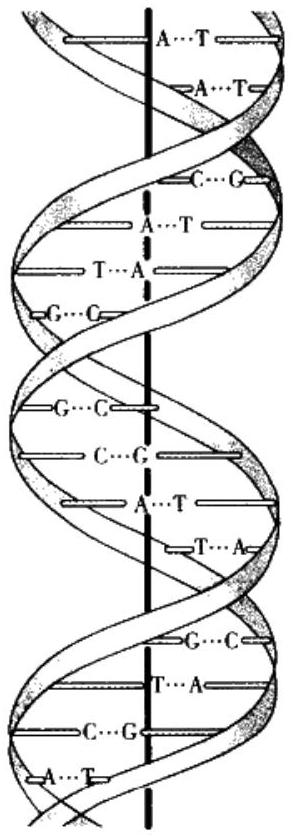
\includegraphics[width=\textwidth]{images/2025_05_15_6a28331d5e7c993ad07ag-590.jpg}

图 13-1 一个互补的双螺旋的示意图。两个糖一磷酸盐的脊椎在外面卷曲着。平躺着的基组成核,它们成对出现——A 总是和 $\mathbf{T}$ 连接, $\mathbf{C}$ 总是和 $\mathbf{G}$ 连接。该结构形成一个螺旋楼梯,成对的基形成胗梯。\\
摘自于 J.D.Watson,The Double Helix.p.130,这里的引用得到版权所有人 G.S.斯坦特的同意。

5 和 6.演绎和检验结果。假说已经形成,接着要对它进行检验。首先,直接的推论是:如果华生和克瑞克提出的双螺旋确实是对 DNA 的正确解释,那么,构造这样一个三维的双螺旋模型是可能的,即所有基都被安排在内部,并且螺旋的角度以及链条的其他特点应当符合以前的 X 光图像及其他的实验结果。这个模型很快就得到了。

许多其他的理论推论被得到,每一个推论的检验都获得了成功。令分子生物学家长期困扰和沮丧的某些数据,由于这样的分析而得以理解。人们了解到,来自于父母的生殖细胞中的 DNA 数量,在普通细胞中只发现了一半。现在我们清楚了个中原因:如果双螺旋在生殖过程中裂开,来自于双亲的裂开的细胞自然只包含正常 DNA 数量的一半。华生一克瑞克对 DNA 结构的解决的正确性的证据迅速增加;不久,他们的假说非常充分

地得到证实。\\
7.应用。华生-克瑞克关于 DNA 结构 128 页的报告\cite{watson1953} 创造了科学史,它对生物学进程的改变是巨大的也是持久的。该知识的广泛且威力强大的运用将他们的成就推到顶峰。在随后的几十年里,人们认识了 DNA序列中使用的编码;整个人类基因组的完整图实际上是完全的,不久人类将得到该图。将 DNA 链进行切割、重组的技术已经得到发展,它们已经在新药、疫苗和人造荷尔蒙的制造中普遍地得到应用。重新组合 DNA 技术仅在 DNA 结构被最终解决的条件下才是可能的,该技术的应用使生物学和医学发生革命,并且仍保持着旺盛的应用生命力。 

\begin{center}
\fbox{\parbox{0.95\textwidth}{
\textbf{本节要点}
\begin{itemize}
\item \textbf{DNA结构发现案例分析}:
  \begin{itemize}
  \item 沃森和克里克的研究遵循了科学研究的七个基本阶段
  \item 与理论模式不同,实际研究中各阶段常交错进行
  \item 成功研究体现了从问题确定到最终说明的完整逻辑过程
  \end{itemize}
\item \textbf{研究起点与发展}:
  \begin{itemize}
  \item 从基因遗传物质问题出发,逐步聚焦于DNA结构
  \item 初始假说:遗传信息在DNA结构中被携带
  \item 多源数据收集与分析,包括X射线衍射图和查尔格夫规则
  \end{itemize}
\item \textbf{科学突破的关键因素}:
  \begin{itemize}
  \item 创造性思维与模型构建相结合
  \item 对已有理论的质疑与修正(基的互补性匹配)
  \item 科学合作与竞争并存的研究环境
  \end{itemize}
\item \textbf{发现的影响与应用}:
  \begin{itemize}
  \item DNA双螺旋结构解释了遗传信息的存储与复制机制
  \item 发现为分子生物学领域带来革命性变革
  \item 应用扩展到基因组测序、新药开发等众多领域
  \end{itemize}
\end{itemize}
}}
\end{center}